\chapter{Proposed Sintactic and Semantic Analyzer}
\label{ch:proposed-sintactic-semantic-analyzer}

Once all the objectives and requirements to be achieved have been described,
the different systems and techniques existing to achieve them have been studied,
and their contributions and shortcomings have been evaluated, we will describe
the proposed solution both in terms of design and possible implementation

\section{Structure}
The system is divided into components so that each component works on its input
and produces its output. In this way, a parser is achieved that behaves like
an API where each element can be called individually. \cref{fig:shex-lite-sema}
shows the different components of this analyzer.

\begin{figure}
    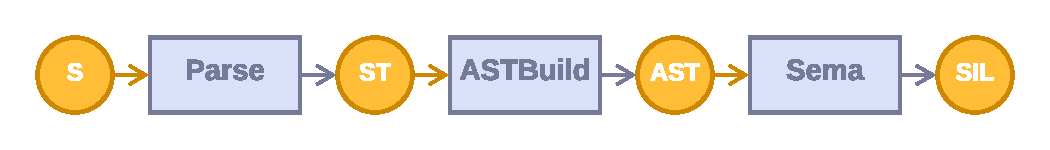
\includegraphics[width=\textwidth]{images/shex-lite-sema.pdf}
    \centering
    \caption[Sintactic and Semantic Analyzer structure]{Sintactic and Semantic Analyzer structure. $S$
    is the Source file. $ST$ is the Syntax Tree. $AST$ is the Abstract Syntax Tree. And $SIL$ is the
    Intermediate Language.}
    \label{fig:shex-lite-sema}
\end{figure}

\subsection{Parse}
The parsing stage occurs from when we find the source code until we produce the
validated syntax tree. This implies that the \textit{lexer}, the \textit{parser} and the \textit{syntactic
validator} influence this stage. 

The general idea of this stage is that you take the source code as input and build a syntactic tree with all
the possible information from the source code. This implies that the syntactic tree is not only made up of
abstract grammar, but also of separators, braces and keywords. \cref{fig:shex-lite-st} shows an example
of the first 20 nodes generated by the parser. There we can see this composition of separators, keywords, braces
and content.

\begin{figure}
    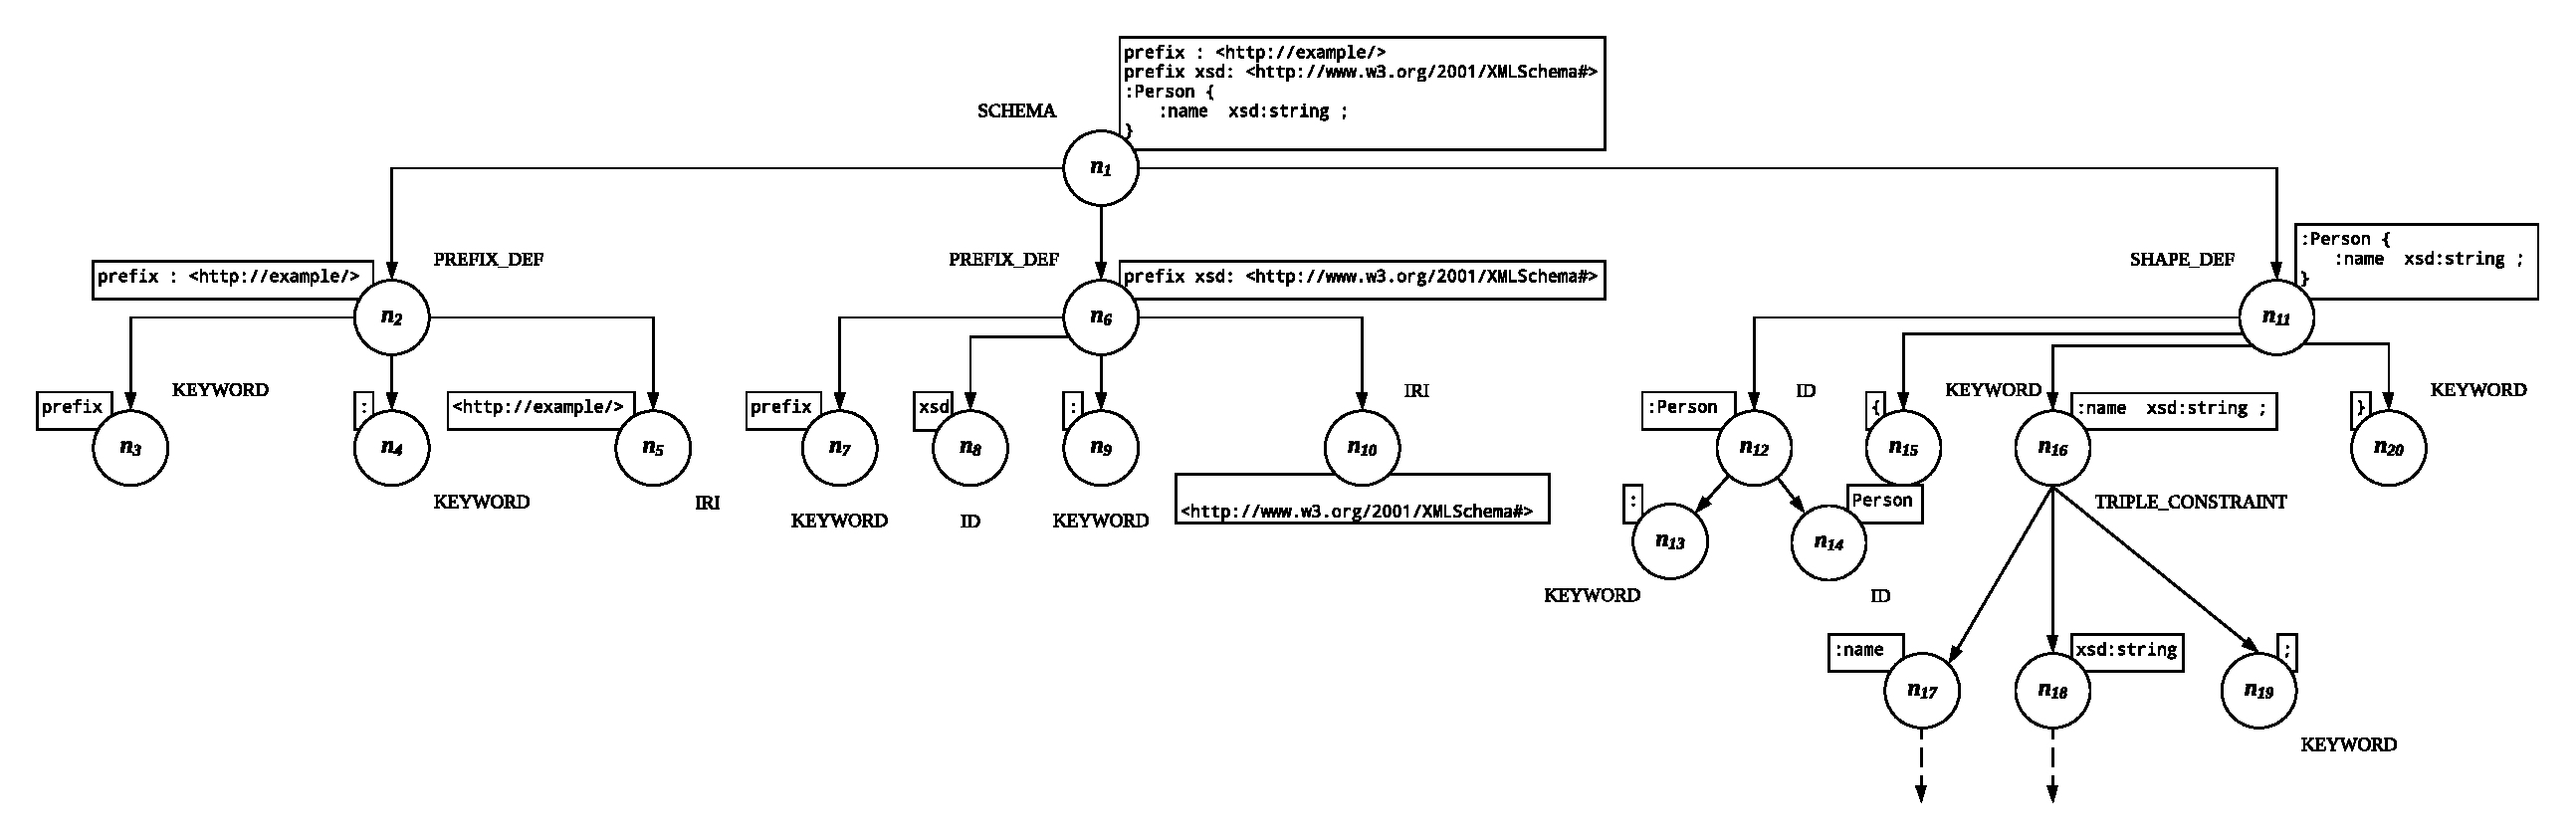
\includegraphics[width=\textwidth]{images/shex-lite-syntax-tree.pdf}
    \centering
    \caption[Syntax Tree tweenty first nodes produced by the parser]{Syntax Tree tweenty first nodes produced by the parser.}
    \label{fig:shex-lite-st}
\end{figure}

Once we have the complete syntactic tree generated, we can go through it to carry out syntactic analysis on the different elements.
For example, in the tree in \cref{fig:shex-lite-st} we could implement a validator that in the event that the last triple constraint
of a shape definition \textit{(node 16)} did not have the semicolon termination keyword \textit{(node 19)}, it would generate a
warning message to the user.

\subsection{Semantic Analyzer}
The semantic analyzer is responsible of building all the possible relations between the AST nodes, analyze and check that
all those relations that must exist indeed exist. For this porpouse as just seen we reduce our Syntax Tree to an
Abstract Syntax Tree. \cref{fig:shex-lite-sema-anal} Shows a the resulting AST after the correspinding analysis and
transformations, we call this graph the \textit{Intermediate Language}.

\begin{figure}
    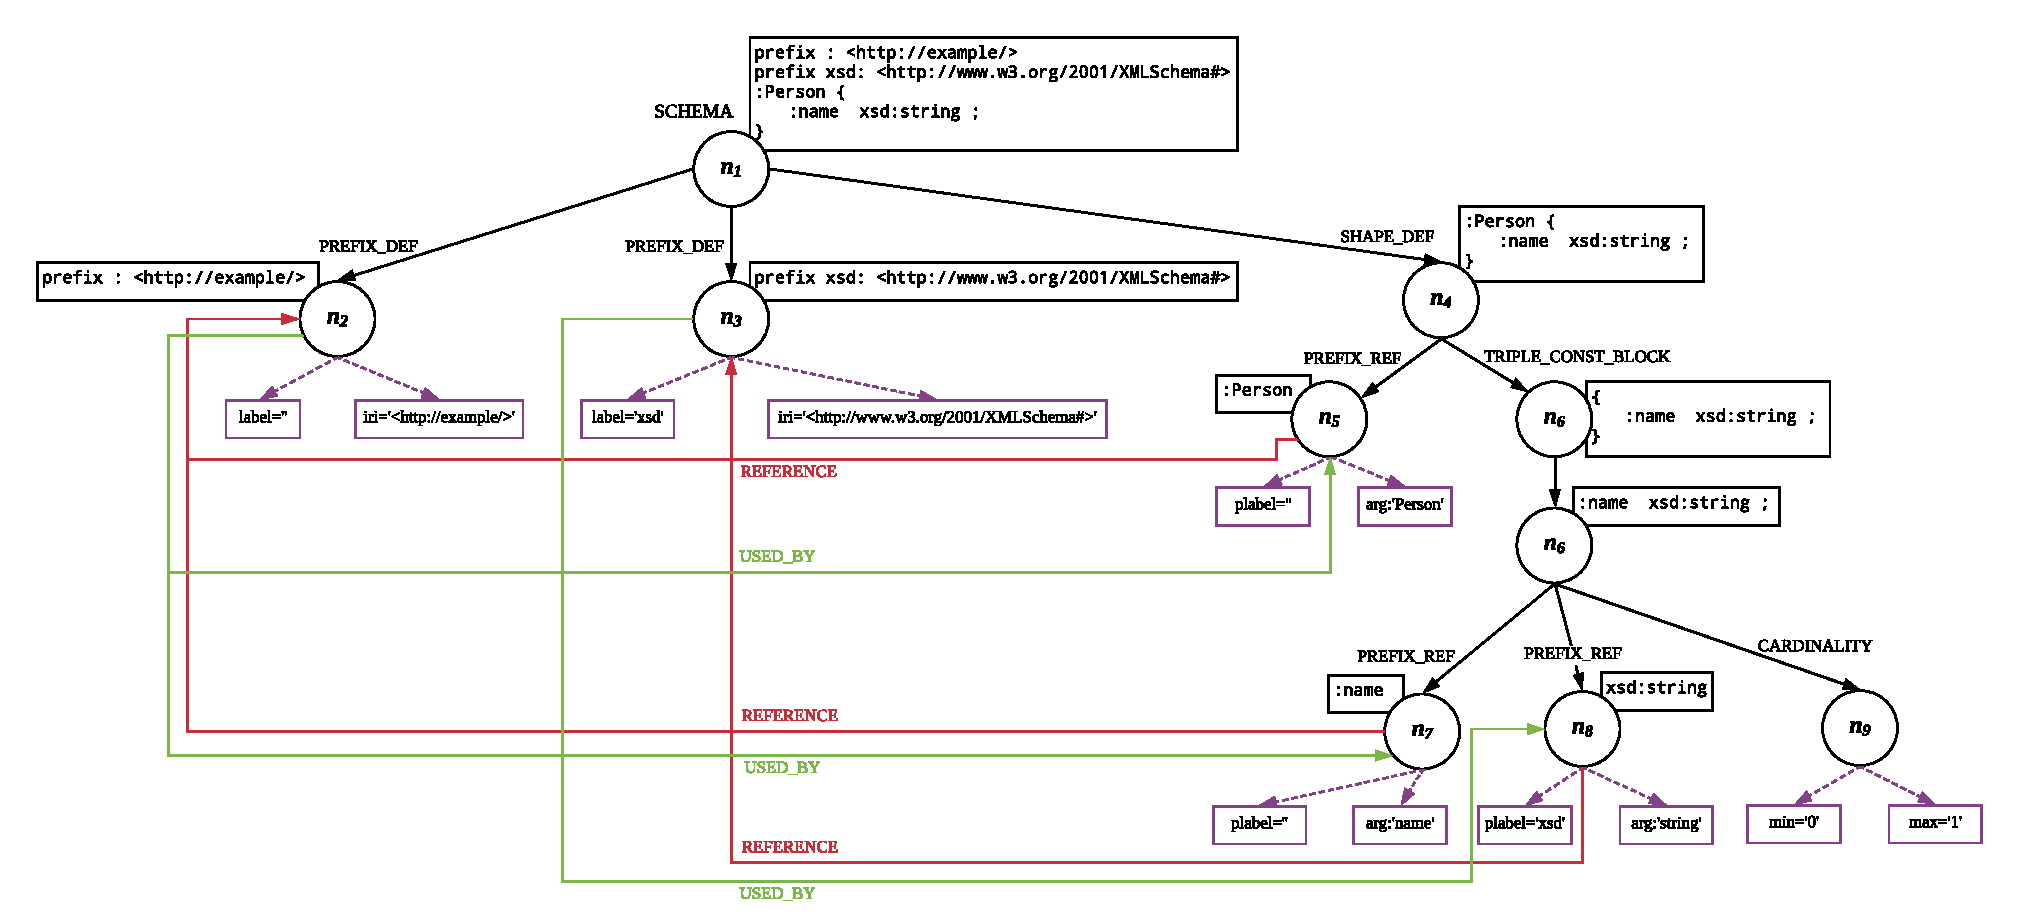
\includegraphics[width=\textwidth]{images/shex-lite-sema-anal.pdf}
    \centering
    \caption[Abstract Syntax Tree produced after validation and transformations]{Abstract Syntax Tree produced after validation and
    transformations.}
    \label{fig:shex-lite-sema-anal}
\end{figure}

Once we have the representation modeled and this representation is capable of expressing all the assumptions of our language,
we can begin to apply validators on our structure. For example if we wanted to find broken references we could go to the nodes
that are a reference to definitions like nodes $n_{\:5,\:7\:and\:8}$ and check that there is indeed a valid reference for each of them.

Furthermore, we can even analyze how many times a definition is used by a reference so that we can launch messages warning the end user
in some cases, such as when a prefix is not used.

\section{Implementation}
As a prove of concept of such a proposals we ofer an implementation for both of them in to a single analyzer. This analyzer is an API
that allows to call separatly the sintactic and the semantic analysis, being the input of the semantic analysis the output of the
sintactic analysis.

The implementation, like the structure, is defined in different parts, parsing, syntactic analysis, AST construction and AST analysis.
In addition to producing errors / warnings.

\subsection{Sintactic Analizer}
To accelerate the development of the system, the Antlr \cite{parr1995antlr} tool has been used to generate syntactic analyzers from a grammar.
In our case the grammar is simply the translation of the starting base grammar \textit{(ShEx micro Compact Syntax)} into the Antlr
syntax. It is important to remark that Antlr by itself is designed to produce ASTs, but we trickle the grammar so it produces
a Tree with all the sintactic information of the program, the Antlr generated tree is identical to the one from \cref{fig:shex-lite-st}.
And from this figure if we can implement the validators as for example the one from \cref{fig:checker-example}.

\begin{figure}
    \begin{lstlisting}[language=Java,numbers=left,basicstyle=\ttfamily\scriptsize]
override def visitConstraint_triple_expr(...) {
  if(/*No trailing semicolon*/)
    //Warn user about this bad practice
}
    \end{lstlisting}
    \caption[Checker implementation for missing semicolons warning generation]{Checker implementation for missing semicolons warning generation.}
    \label{fig:checker-example}
\end{figure}


\section{Detected Erasures}